\begin{figure*}[!hbt]
  \centering
  \subfigure[Speedup with varying Prune tolerance $\tau_p$]{
    \label{fig:adjust-prune--speedup}
    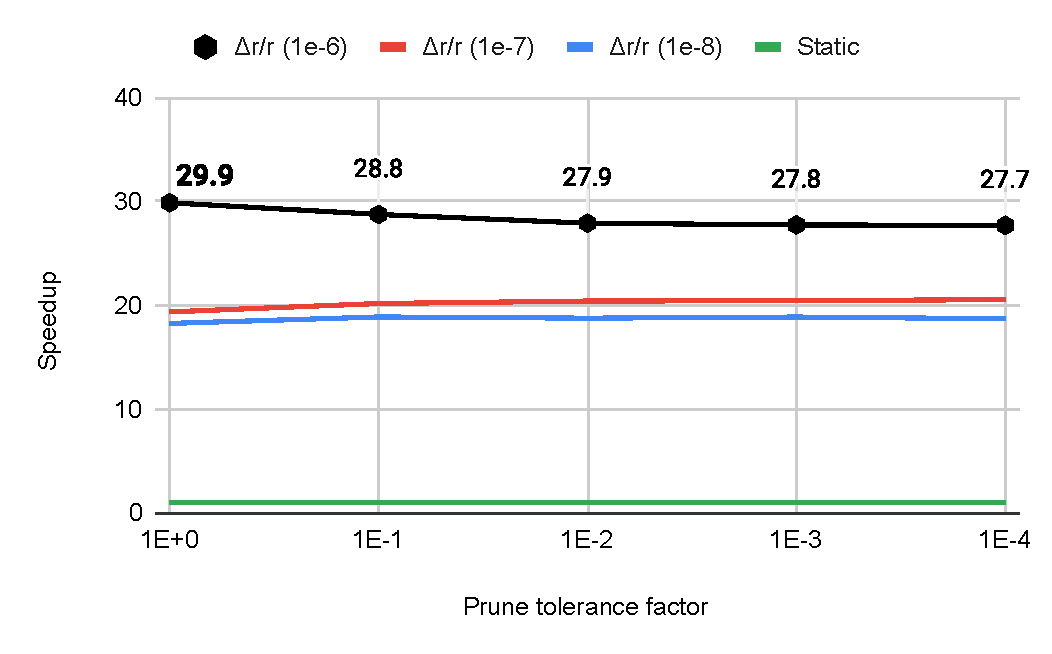
\includegraphics[width=0.48\linewidth]{out/adjust-prune-speedup.pdf}
  }
  \subfigure[Error in ranks obtained with varying Prune tolerance $\tau_p$]{
    \label{fig:adjust-prune--error}
    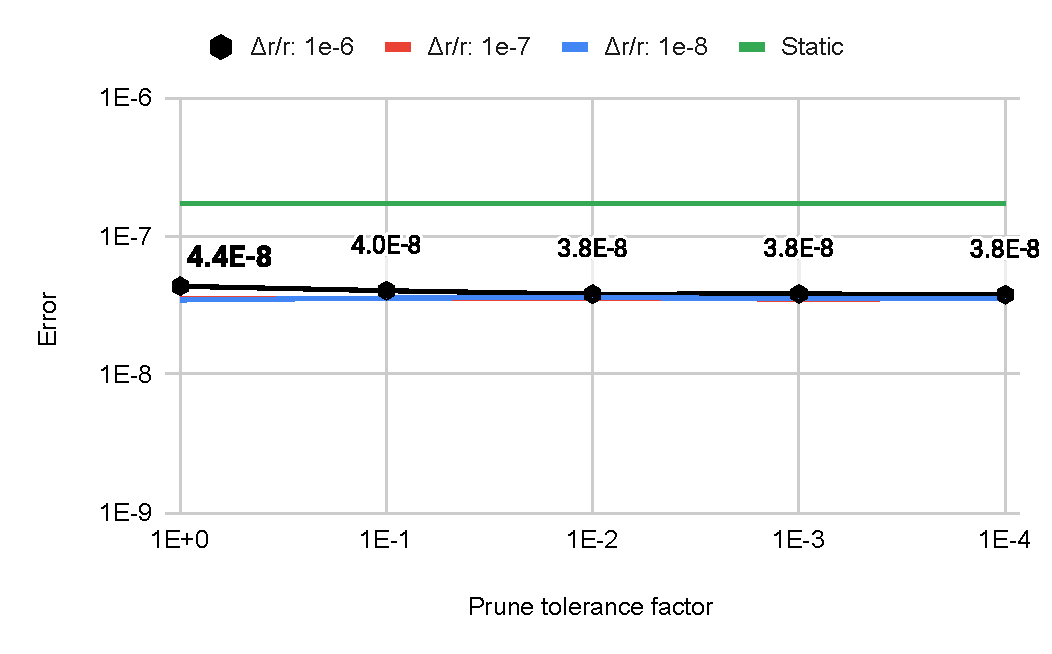
\includegraphics[width=0.48\linewidth]{out/adjust-prune-error.pdf}
  } \\[-2ex]
  \caption{Mean Speedup and Error in ranks obtained, with varying prune tolerance $\tau_p$ from $\tau_f$ to $\tau_f/10^5$, using the optimal approach of expanding frontier, i.e., expanding frontier based on relative change in rank $\Delta r/r$ of a vertex with a frontier tolerance $\tau_f$ of $10^{-6}$. In addition to a frontier tolerance $\tau_f$ of $10^{-6}$, we also experiment with $\tau_f$ values of $10^{-7}$ and $10^{-8}$. We also include the mean speedup and error in ranks obtained with Static PageRank as a reference. The $\Delta r/r$ approach with a frontier tolerance $\tau_f$ of $10^{-6}$ and a prune tolerance $\tau_p$ of $\tau_f = 10^{-6}$ performs the best, with lower error than Static PageRank.}
  \label{fig:adjust-prune}
\end{figure*}

\ignore{Mean Speedup and Error in ranks obtained (with respect to ranks obtained with Reference Static PageRank) with the best approach of expanding frontier, i.e., marking outgoing neighbors as affected, based on relative change in rank $\Delta r/r$ of a vertex, with a frontier tolerance $\tau_f$ of $10^{-6}$. In the figure, we vary prune tolerance $\tau_p$ from $\tau_f$ to $\tau_f/10^5$. When the relative change in rank of a vertex falls within prune tolerance $\tau_p$, we mark the vertex as not affected. In addition to a frontier tolerance $\tau_f$ of $10^{-6}$, we also experiment with a $\tau_f$ of $10^{-7}$ and $10^{-8}$. We also include the mean speedup ($1$) and error in ranks obtained ($1.7\times10^{-7}$) with Static PageRank as a reference. Here, $\Delta r$ is the change in rank of a vertex and $r$ represents the rank of the vertex (it is actually the \texttt{max} of the previous and the current rank value of the vertex). This figure indicates that the $\Delta r/r$ approach with a frontier tolerance $\tau_f$ of $10^{-6}$ and a prune tolerance $\tau_p$ of $\tau_f = 10^{-6}$ performs the best, while obtaining ranks with lower error than Static PageRank.}
